\subsection{sort\_data() и get\_sorted\_array()}

Блок-схема на рисунках \ref{fig:sort_data_sort_data} и \ref{fig:sort_data_get_sorted_array}.

\begin{figure}[p]
    \center{
        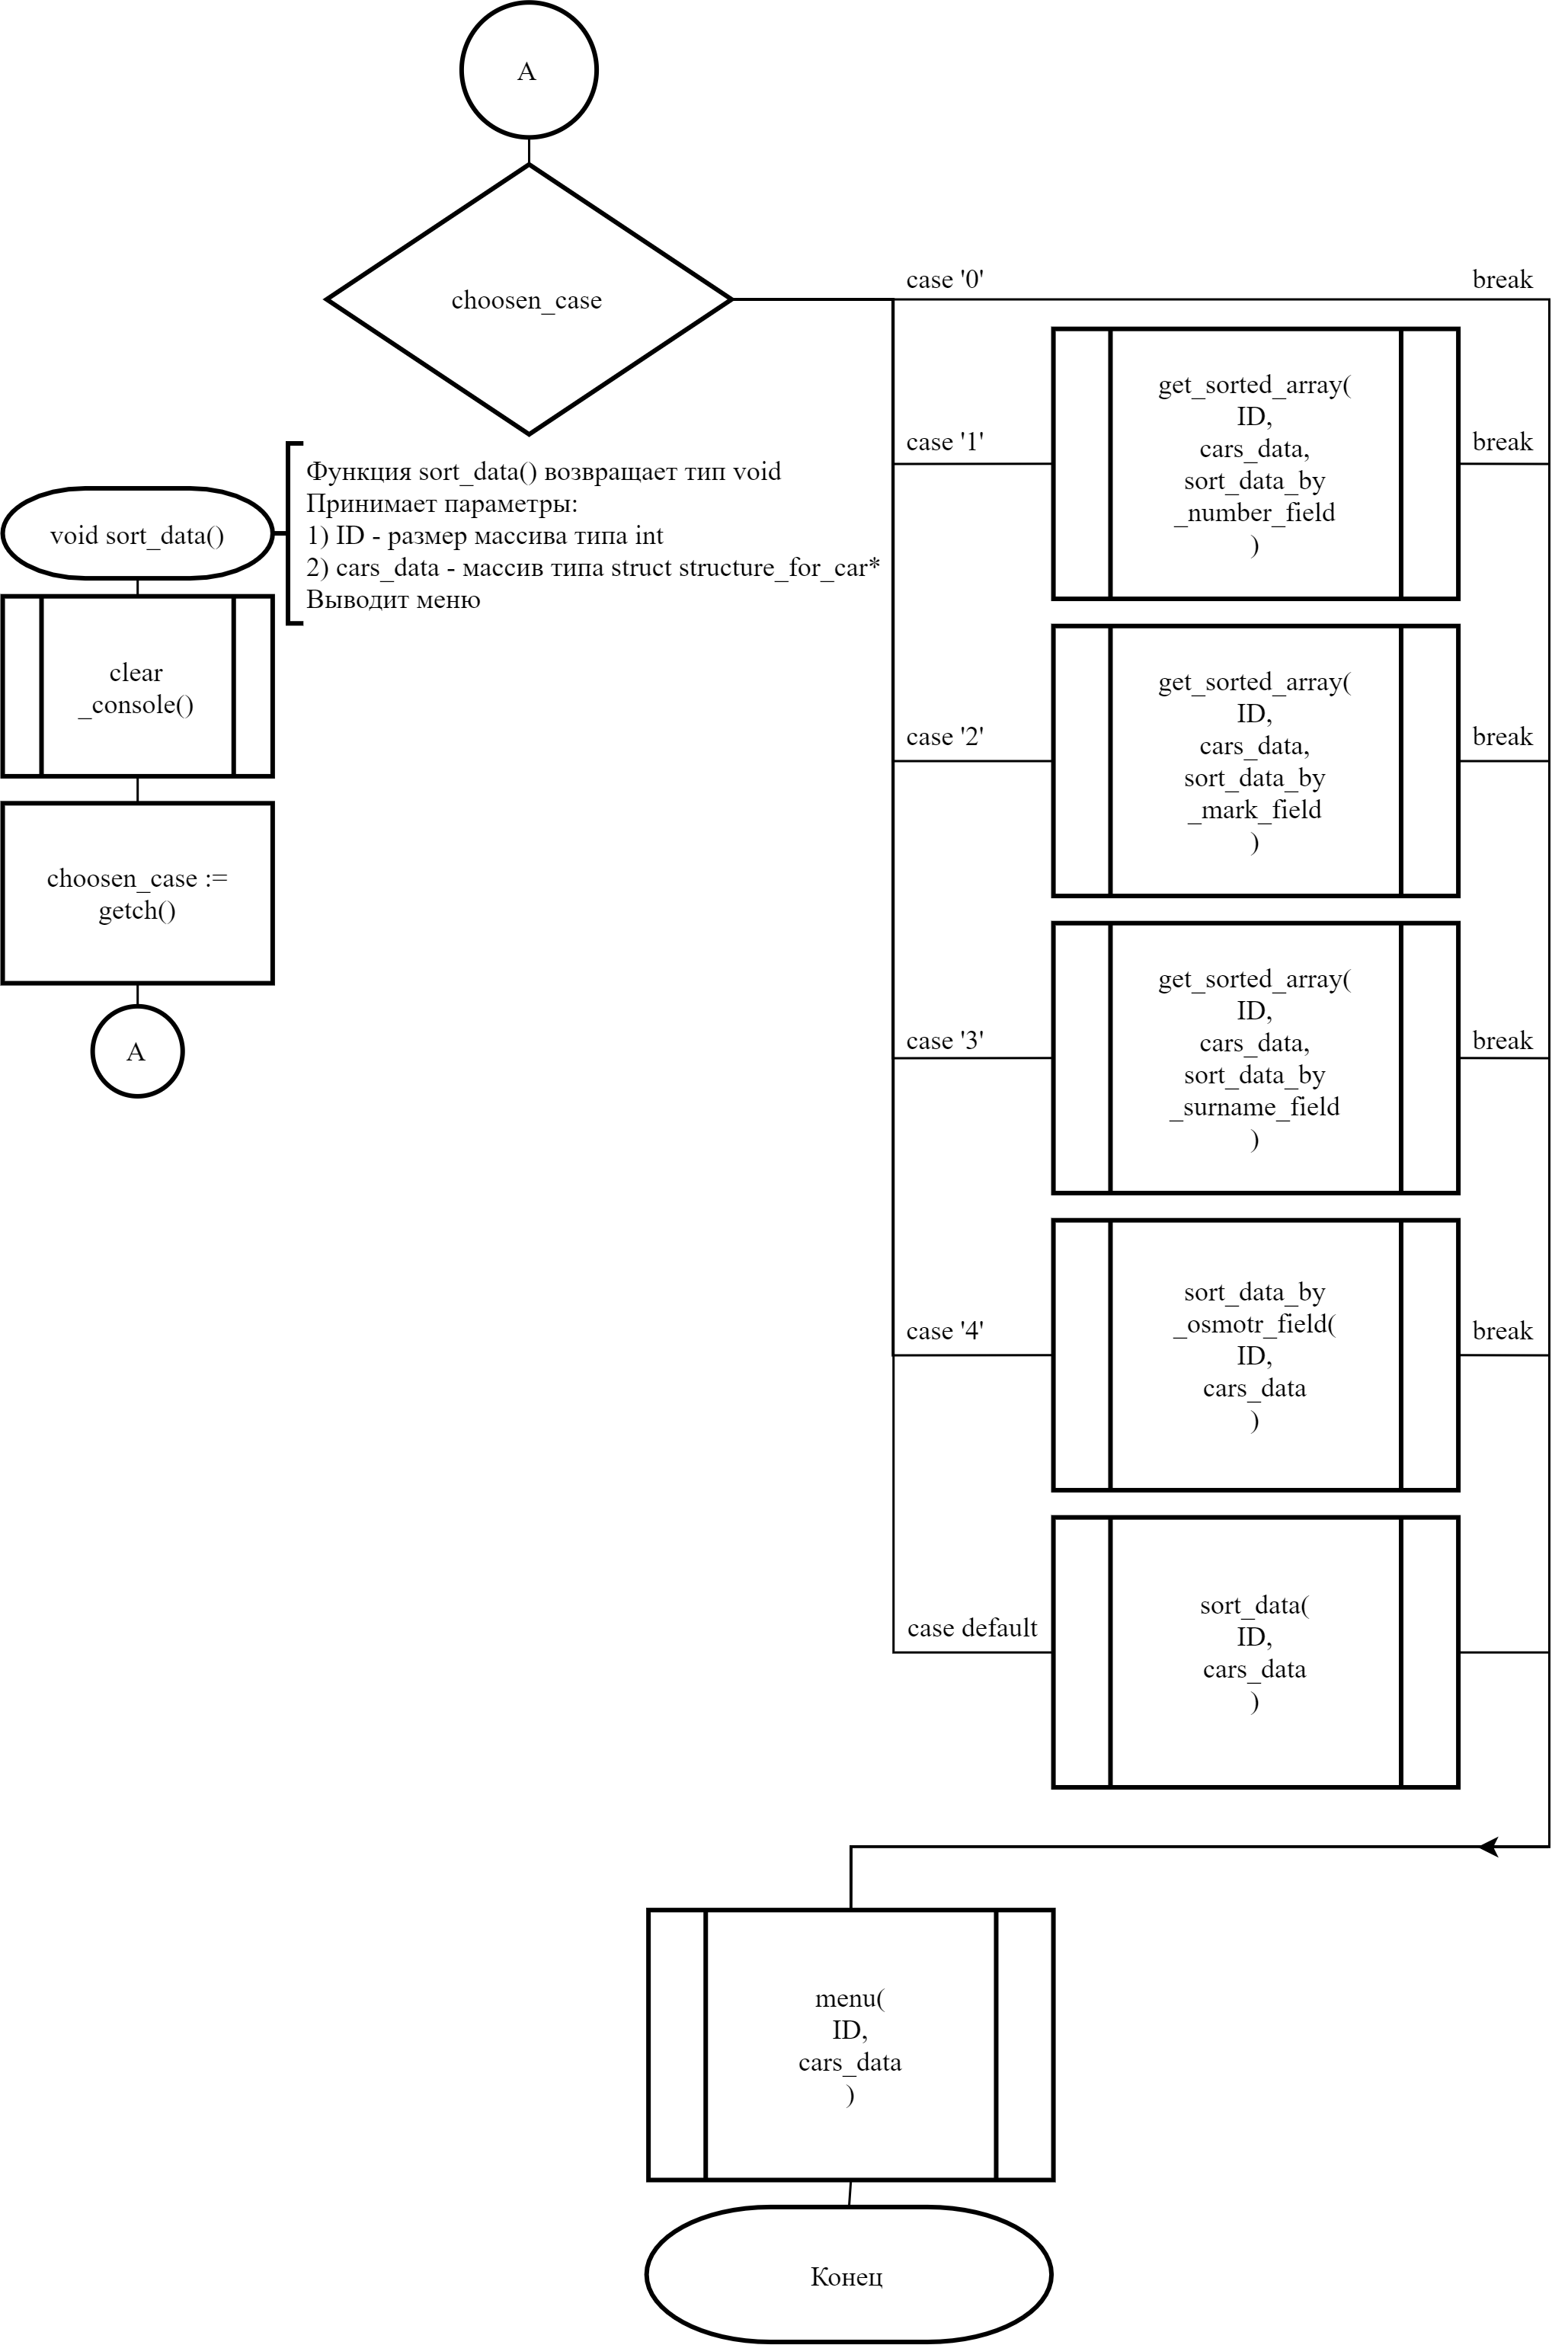
\includegraphics[]{../13/src/lab/menu/sort_data/sort_data-sort_data.png}
    }
    \caption{sort\_data()}
    \label{fig:sort_data_sort_data}
\end{figure}

\begin{figure}[p]
    \center{
        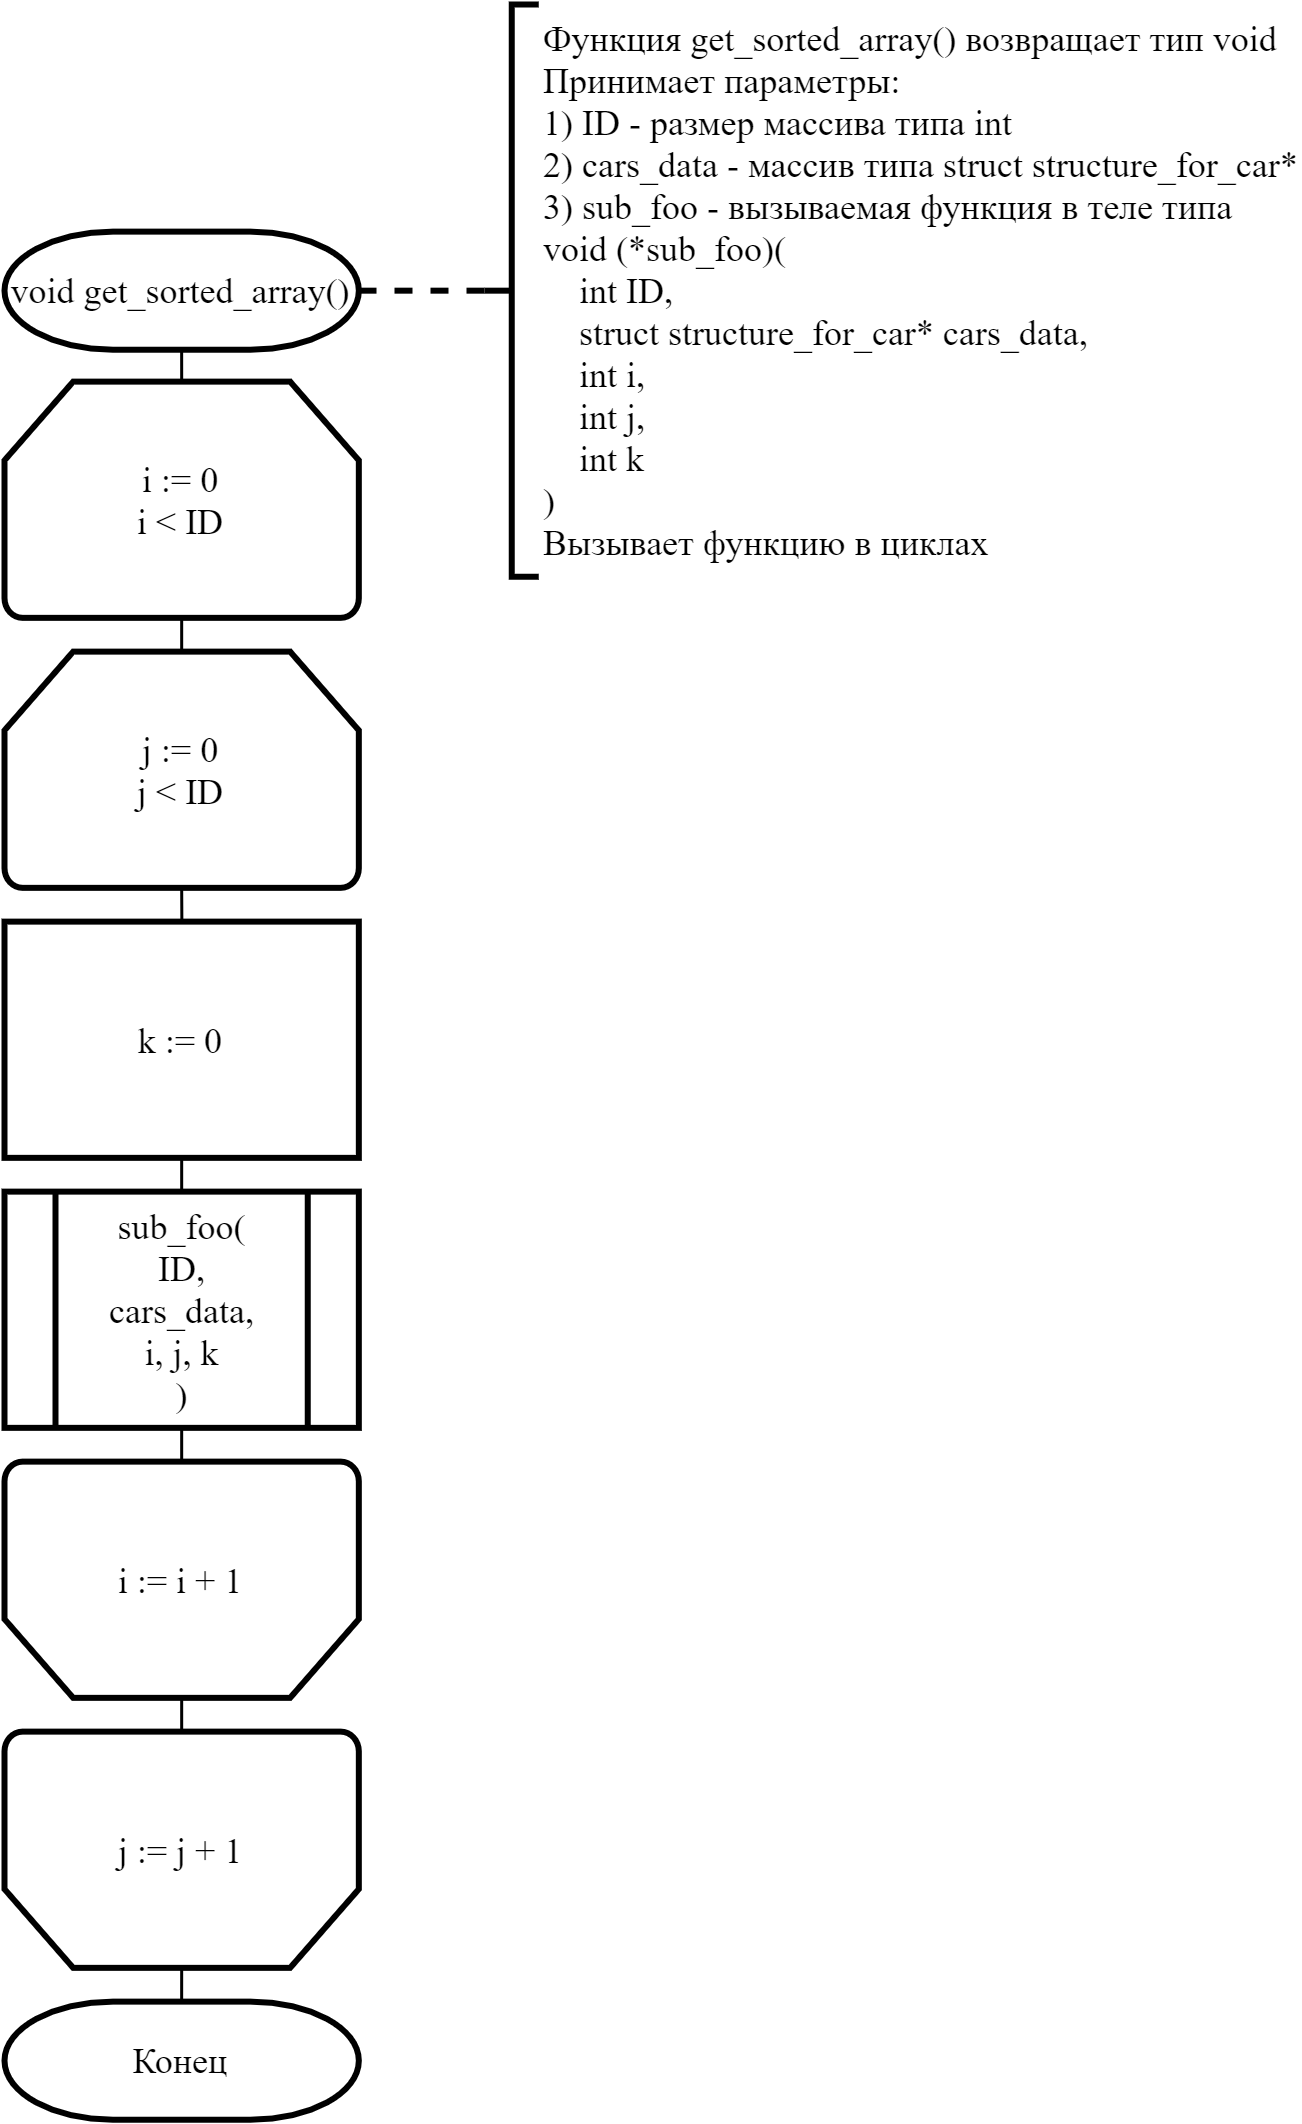
\includegraphics[]{../13/src/lab/menu/sort_data/sort_data-get_sorted_array.png}
    }
    \caption{get\_sorted\_array()}
    \label{fig:sort_data_get_sorted_array}
\end{figure}

\lstinputlisting[
    language=C,
    name=sort\_data.h
]{../13/src/lab/menu/sort_data/sort_data.h}

\lstinputlisting[
    language=C,
    name=sort\_data.c
]{../13/src/lab/menu/sort_data/sort_data.c}

\newpage